% Template GRASS newsletter - Article
% Language: Latex
%

% Head

\title{Manuel pour d\'ebuter avec le SIG GRASS}
\subtitle{GRASS en version originale}
\author{GRASS Development Team}

\maketitle

\section{Introduction}

Cette capture d'\'ecran est le SIG GRASS en version original sous Windows
(http://geni.ath.cx/grass.html).Fig.~\ref{fig:grass000}
%\setkeys{Gin}{width=1\textwidth}
\begin{figure}[htbp]
   \centering
   %name of your graphic, without the path AND in PNG (screnshots etc)/PDF (drawings) format:
   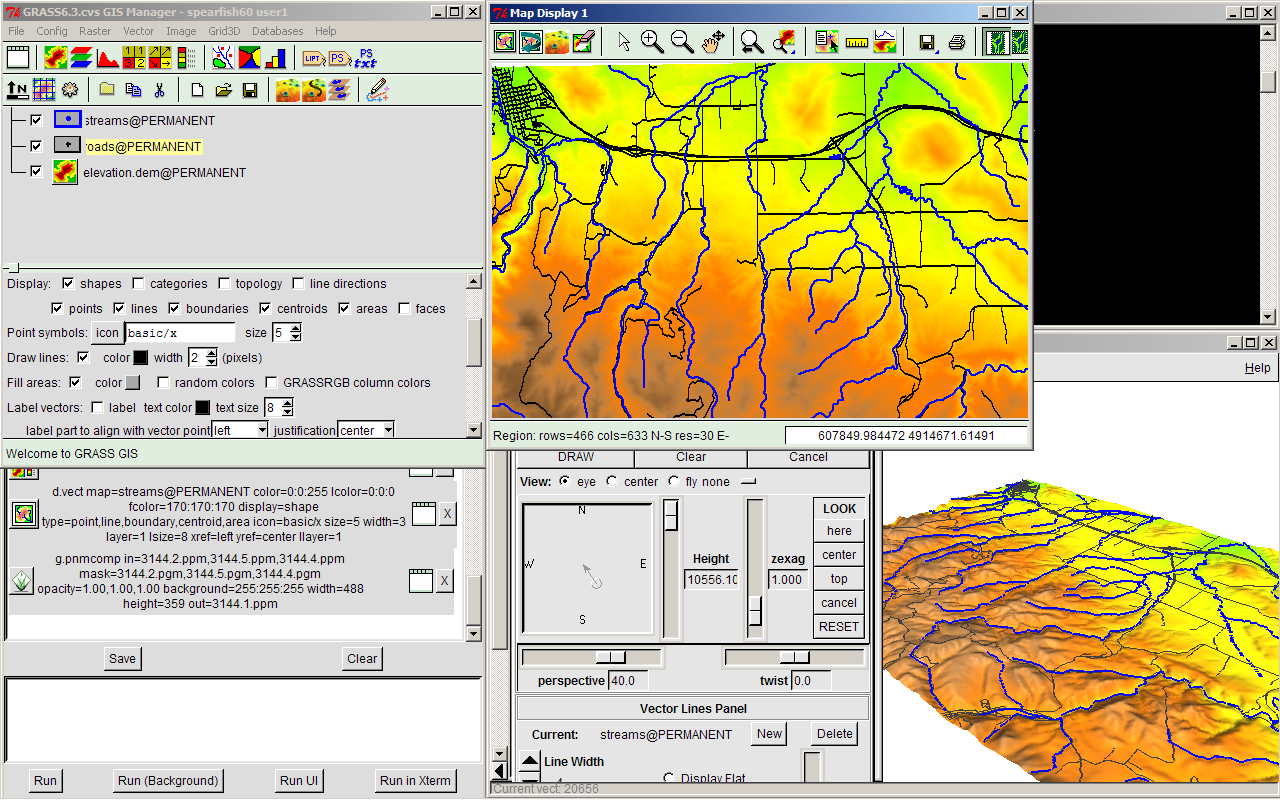
\includegraphics[scale=0.15]{grass000.png}
   %caption of the figure
   \caption{GRASS en version original sous Windows}
   %label of the figure, which has to correspond to \ref{}:
   \label{fig:grass000}
\end{figure}

Lancer le SIG GRASS: S\'electionnez la Location Spearfish60 et cliquez sur
``Enter GRASS'':Fig.~\ref{fig:grass001}

%\setkeys{Gin}{width=1\textwidth}
\begin{figure}[htbp]
   \centering
   %name of your graphic, without the path AND in PNG (screnshots etc)/PDF (drawings) format:
   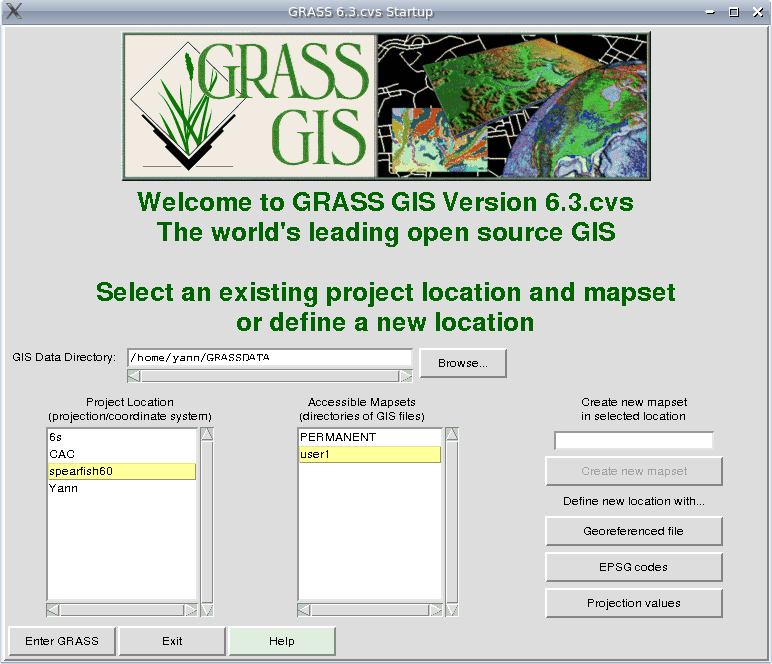
\includegraphics[scale=0.3]{grass001.png}
   %caption of the figure
   \caption{Ecran d'acceuil}
   %label of the figure, which has to correspond to \ref{}:
   \label{fig:grass001}
\end{figure}

A ce moment cel\`a devrait ressembler \`a: Fig.~\ref{fig:grass002}

%\setkeys{Gin}{width=1\textwidth}
\begin{figure}[htbp]
   \centering
   %name of your graphic, without the path AND in PNG (screnshots etc)/PDF (drawings) format:
   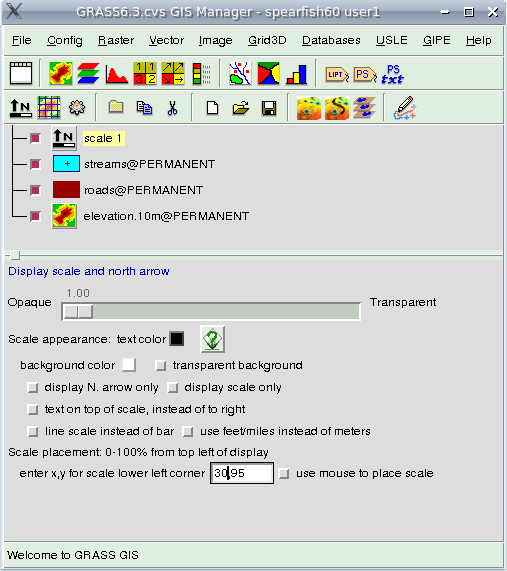
\includegraphics[scale=0.35]{grass002.png}
   %caption of the figure
   \caption{Gestionnaire du SIG}
   %label of the figure, which has to correspond to \ref{}:
   \label{fig:grass002}
\end{figure}

Plus d'information sur le GUI se trouve dans l'appendice A \ref{appendixA}.

Chargez la couche elevation.10m en cliquant sur le bouton de d'affichage raster (second bouton \`a partir de gauche):Fig.~\ref{fig:grass003}

%\setkeys{Gin}{width=1\textwidth}
\begin{figure}[htbp]
   \centering
   %name of your graphic, without the path AND in PNG (screnshots etc)/PDF (drawings) format:
   
\includegraphics[scale=0.5]{grass003.png}
   %caption of the figure
   \caption{Affichage \'el\'ementaire}
   %label of the figure, which has to correspond to \ref{}:
   \label{fig:grass003}
\end{figure}

Une fois s\'electionn\'e, l'interface d'utilisation de GRASS aura une nouvelle couche comme cell-ci:Fig.~\ref{fig:grass004}

%\setkeys{Gin}{width=1\textwidth}
\begin{figure}[htbp]
   \centering
   %name of your graphic, without the path AND in PNG (screnshots etc)/PDF (drawings) format:
   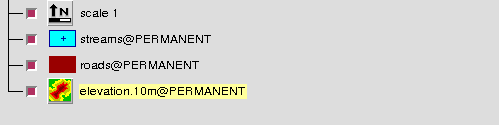
\includegraphics[scale=0.35]{grass004.png}
   %caption of the figure
   \caption{}
   %label of the figure, which has to correspond to \ref{}:
   \label{fig:grass004}
\end{figure}

En s\'electionnant la nouvelle couche, vous aurez acc\`es \`a un menu contextuel comme ceci:Fig.~\ref{fig:grass005}

%\setkeys{Gin}{width=1\textwidth}
\begin{figure}[htbp]
   \centering
   %name of your graphic, without the path AND in PNG (screnshots etc)/PDF (drawings) format:
   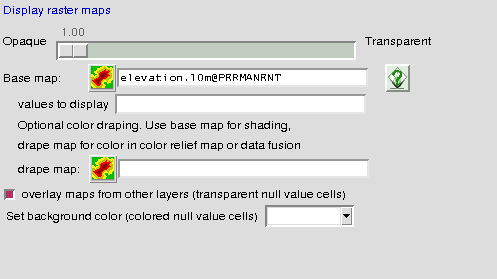
\includegraphics[scale=0.35]{grass005.png}
   %caption of the figure
   \caption{}
   %label of the figure, which has to correspond to \ref{}:
   \label{fig:grass005}
\end{figure}

Ajoutez une couche vectorielle en utilisant la 8\`eme ic\^one \`a partir de la gauche. Fig.~\ref{fig:grass006}

%\setkeys{Gin}{width=1\textwidth}
\begin{figure}[htbp]
   \centering
   %name of your graphic, without the path AND in PNG (screnshots etc)/PDF (drawings) format:
   
\includegraphics[scale=0.5]{grass006.png}
   %caption of the figure
   \caption{}
   %label of the figure, which has to correspond to \ref{}:
   \label{fig:grass006}
\end{figure}

Ajoutez une couche vectorielle "stream" (de couleur bleue) et "road" de couleur amrron. Ci-dessous est l'exemple pour "stream" Fig.~\ref{fig:grass007}

%\setkeys{Gin}{width=1\textwidth}
\begin{figure}[htbp]
   \centering
   %name of your graphic, without the path AND in PNG (screnshots etc)/PDF (drawings) format:
   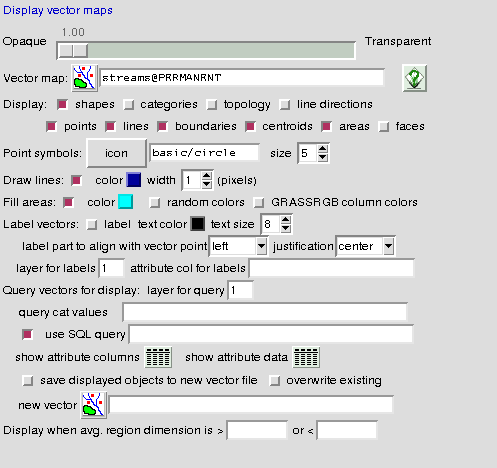
\includegraphics[scale=0.45]{grass007.png}
   %caption of the figure
   \caption{}
   %label of the figure, which has to correspond to \ref{}:
   \label{fig:grass007}
\end{figure}

Le r\'esultat devrait \^etre comme ceci (plus ou moins):Fig.~\ref{fig:grass008}

%\setkeys{Gin}{width=1\textwidth}
\begin{figure}[htbp]
   \centering
   %name of your graphic, without the path AND in PNG (screnshots etc)/PDF (drawings) format:
   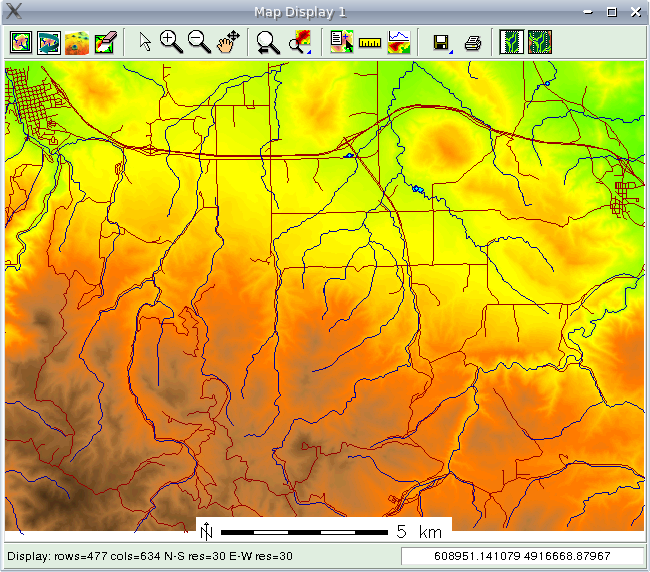
\includegraphics[scale=0.35]{grass008.png}
   %caption of the figure
   \caption{}
   %label of the figure, which has to correspond to \ref{}:
   \label{fig:grass008}
\end{figure}

\section{MANIPULATIONS DE DEM}
Affichage du dem:Fig.~\ref{fig:grass009}

%\setkeys{Gin}{width=1\textwidth}
\begin{figure}[htbp]
   \centering
   %name of your graphic, without the path AND in PNG (screnshots etc)/PDF (drawings) format:
   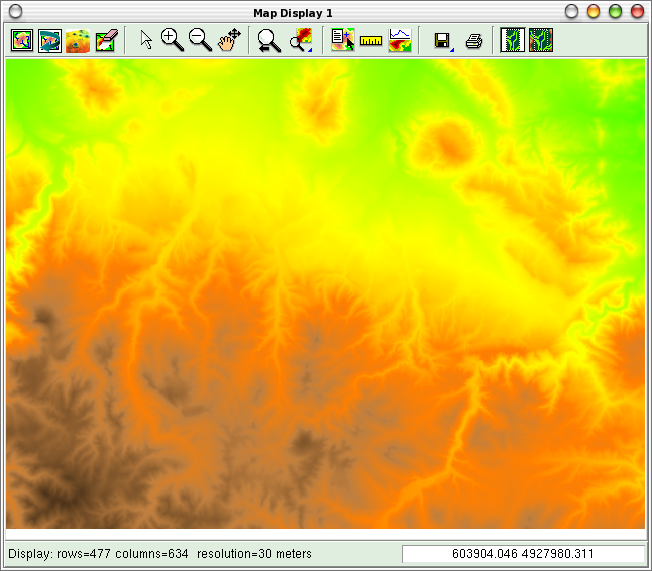
\includegraphics[scale=0.35]{grass009.png}
   %caption of the figure
   \caption{Affichage du DEM}
   %label of the figure, which has to correspond to \ref{}:
   \label{fig:grass009}
\end{figure}

\subsection{Calcul de pente et d'aspect}
Raster/Terrain Analysis/Slope and Aspect. Fig.~\ref{fig:grass010}

%\setkeys{Gin}{width=1\textwidth}
\begin{figure}[htbp]
   \centering
   %name of your graphic, without the path AND in PNG (screnshots etc)/PDF (drawings) format:
   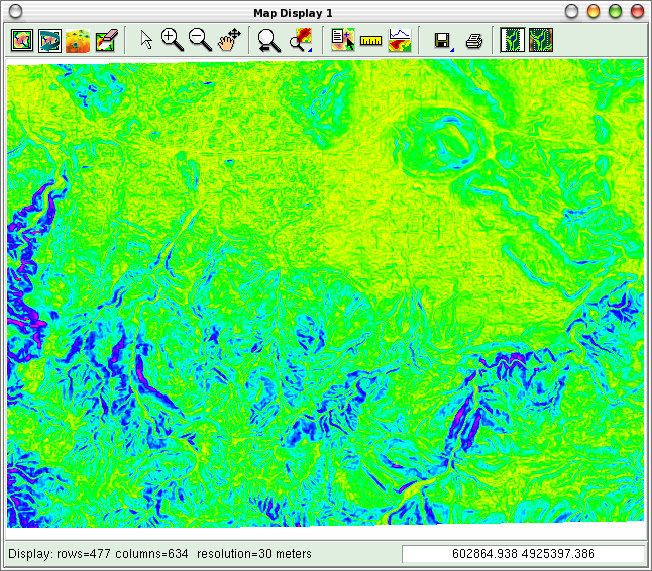
\includegraphics[scale=0.35]{grass010.png}
   %caption of the figure
   \caption{Pente}
   %label of the figure, which has to correspond to \ref{}:
   \label{fig:grass010}
\end{figure}

Calcul de carte de relief ombrag\'e ( prenez Raster/Terrain Analysis/Shaded Relief Map).
La carte de relief ombrag\'e devrait \^etre comme ceci quand la carte "elevation.10m" est superimpos\'ee dessus avec une opacit\'e de 0.75: Fig.~\ref{fig:grass011}

%\setkeys{Gin}{width=1\textwidth}
\begin{figure}[htbp]
   \centering
   %name of your graphic, without the path AND in PNG (screnshots etc)/PDF (drawings) format:
   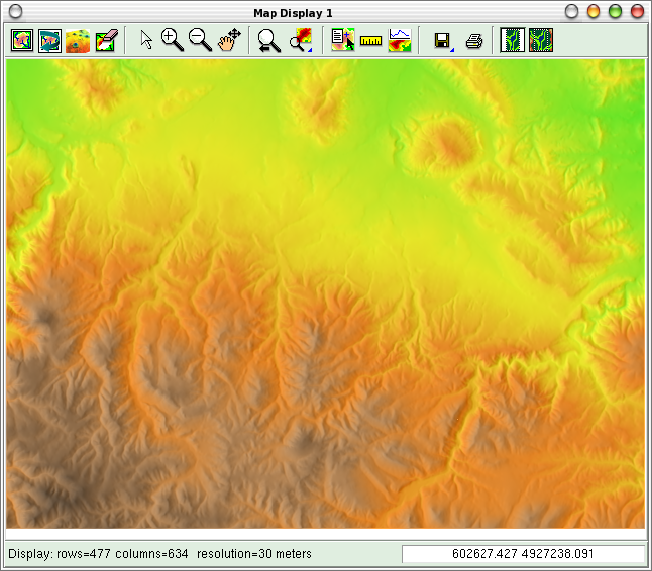
\includegraphics[scale=0.35]{grass011.png}
   %caption of the figure
   \caption{Relief Ombrag\'e}
   %label of the figure, which has to correspond to \ref{}:
   \label{fig:grass011}
\end{figure}

\subsection{Programme d'analyse de basin versant}
Raster/Hydrologic modeling/Watershed Analysis.
Remplissezs les param\`etres d'entr\'e de la carte d'altitude avec ``elevation.10m''. La taille minimum de l'ext\'erieur d'un bassin versant doit \^etre de 5000 pixels. Remplissez les param\`etres de sortie pour toutes les cartes disponibles (i.e. ``\_cells\_nbr'', ``\_drain\_dir'', ``\_drain\_dir'', ``\_basins'', ``\_streams'', ``\_half\_basins'', ``\_visual'', ``\_LS'', ``\_S'').

Voici ce que doit dire l' ex\'ecution du module:

SECTION 1a (of 6): Initiating Memory.

SECTION 1b (of 6): Determining Offmap Flow.

SECTION 2: A * Search. 

SECTION 3: Accumulating Surface Flow.

SECTION 4: Length Slope determination.

SECTION 5: Watershed determination.

SECTION 6: Closing Maps.

La carte r\'esultante ``\_basins'' devrait ressembler \`a cel\`a:Fig.~\ref{fig:grass012}

%\setkeys{Gin}{width=1\textwidth}
\begin{figure}[htbp]
   \centering
   %name of your graphic, without the path AND in PNG (screnshots etc)/PDF (drawings) format:
   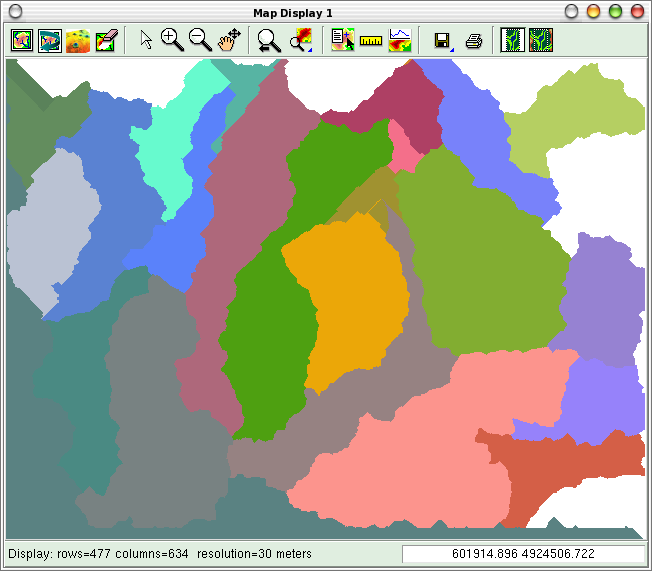
\includegraphics[scale=0.35]{grass012.png}
   %caption of the figure
   \caption{Carte de basins versants}
   %label of the figure, which has to correspond to \ref{}:
   \label{fig:grass012}
\end{figure}


La carte r\'esultante ``\_streams'' devrait ressembler \`a cel\`a: Fig.~\ref{fig:grass013} comparez-l\`a avec la carte vectorielle ``streams''.

%\setkeys{Gin}{width=1\textwidth}
\begin{figure}[htbp]
   \centering
   %name of your graphic, without the path AND in PNG (screnshots etc)/PDF (drawings) format:
   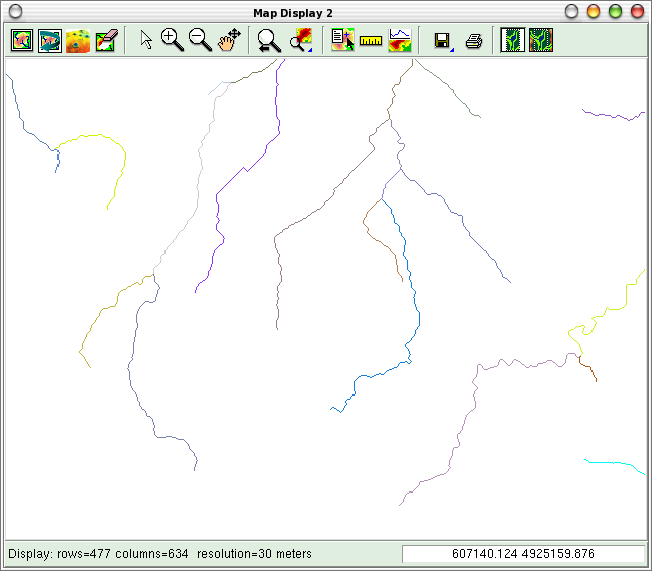
\includegraphics[scale=0.35]{grass013.png}
   %caption of the figure
   \caption{Carte de r\'eseau hydrologique}
   %label of the figure, which has to correspond to \ref{}:
   \label{fig:grass013}
\end{figure}

Relancez avec des valuers diff\'erentes au lieu de 5000 pixels, i.e. 2000 et 10000.
Comparez en vectorisant les r\'eseaux hydrologiques g\'en\'er\'es. La vectorisation suit ces \'etapes:
1-Raster/Neighborhood Analysis/Thin Linear Features
2-File/Map Type Conversion/Raster to Vector Map
3-Vector/Develop Map/Create-Rebuild Topology (optional)

\subsection{Identification de site de station de suivit de la Pollution d'un ruisseau}
En consid\'erant qu'une usine de transformation/traitement de bois fasse une demande de permis pour mettre en place une nouvelle usine dans le basin versant. La localisation est distante du r\'eseau hydrologique majeur cartographi\'e (598713.35(E) 4920069.15(N)), le conseil local vous a employ\'e pour \'evaluer le chemin de quelques effluents mineurs qui pourraient se retrouver dans le r\'eseau majeur \`a partir de l'usine qui va \^etre install\'ee, et sp\'ecialement leurs coordonn\'ees g\'eographiques du point de rencontre o\`u le conseil va mettre en place une station de suivit automatique.
Utilisez Raster/Terrain Analysis/Least Cost Route Or Flow, v\^otre r\'esultat devrait ressembler a cel\`a: Fig.~\ref{fig:grass014}

%\setkeys{Gin}{width=1\textwidth}
\begin{figure}[htbp]
   \centering
   %name of your graphic, without the path AND in PNG (screnshots etc)/PDF (drawings) format:
   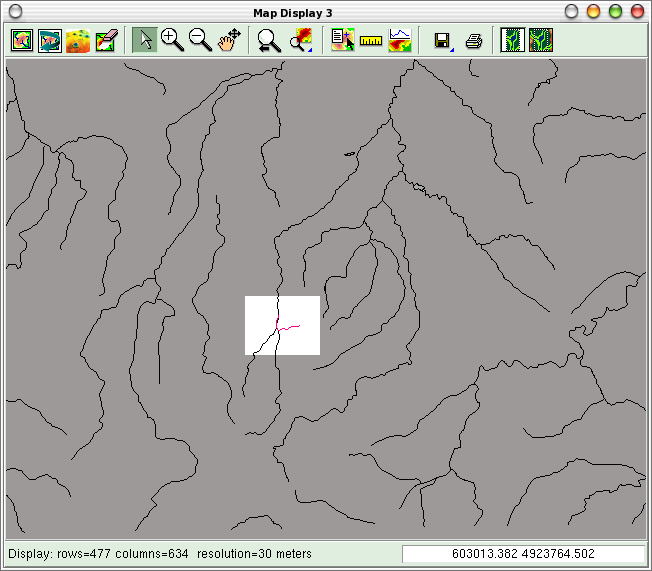
\includegraphics[scale=0.35]{grass014.png}
   %caption of the figure
   \caption{}
   %label of the figure, which has to correspond to \ref{}:
   \label{fig:grass014}
\end{figure}

Quelle est la localisation (Est,Nord) du chemin hydrologique g\'en\'er\'e rejoignant la rivi\`ere cartographi\'ee, et donc lieu propos\'e pour installer une station de suivit?

\section{Analyse d'habitat avec le SIG GRASS}
\subsection{Introduction}

http://www.udel.edu/johnmack/frec682/682proj2.html

Ce cours est disponible en ligne sous le nom ``FREC 682 Spatial Analysis''. Ce mat\'eriel a \'et\'e modifi\'e pour r\'epondre aux changements venant avec GRASS  version 6.3 et additionnelles.

Dans cette session, les \'el\'ements dont vous aurez besoins sont essentiellement (regardez dans la partie RASTER de l'interface principale): 
Le module BUFFERING:   Raster/Create buffers Fig.~\ref{fig:grass015}
Le module MAP CALCULATOR:   Raster/Map Calculator Fig.~\ref{fig:grass016}

%\setkeys{Gin}{width=1\textwidth}
\begin{figure}[htbp]
   \centering
   %name of your graphic, without the path AND in PNG (screnshots etc)/PDF (drawings) format:
   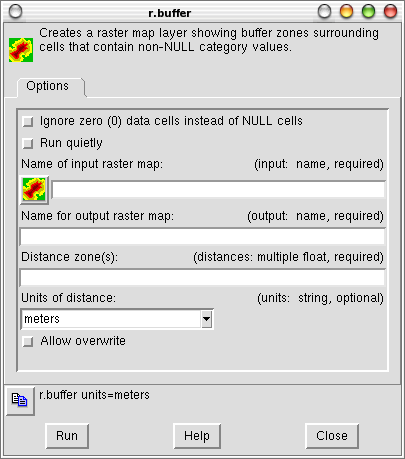
\includegraphics[scale=0.35]{grass015.png}
   %caption of the figure
   \caption{BUFFERING}
   %label of the figure, which has to correspond to \ref{}:
   \label{fig:grass015}
\end{figure}

%\setkeys{Gin}{width=1\textwidth}
\begin{figure}[htbp]
   \centering
   %name of your graphic, without the path AND in PNG (screnshots etc)/PDF (drawings) format:
   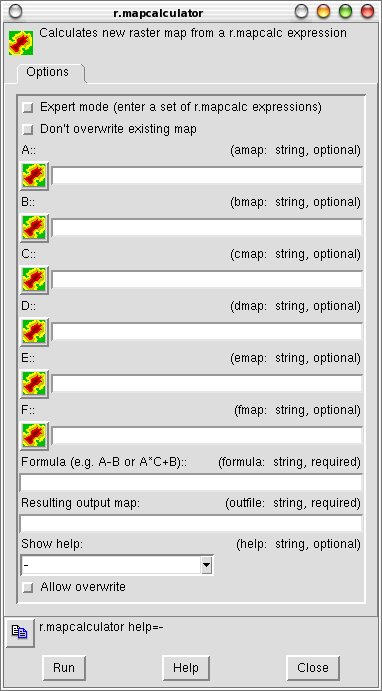
\includegraphics[scale=0.35]{grass016.png}
   %caption of the figure
   \caption{MAP CALCULATOR}
   %label of the figure, which has to correspond to \ref{}:
   \label{fig:grass016}
\end{figure}

Certains modules additionnels pour plus tard

Questionner une carte avec la souris:   
Dans la fen\^etre d'affichage, cherchez:   Fig.~\ref{fig:grass017}

%\setkeys{Gin}{width=1\textwidth}
\begin{figure}[htbp]
   \centering
   %name of your graphic, without the path AND in PNG (screnshots etc)/PDF (drawings) format:
   
\includegraphics[scale=1]{grass017.png}
   %caption of the figure
   \caption{Questionner une carte avec la souris}
   %label of the figure, which has to correspond to \ref{}:
   \label{fig:grass017}
\end{figure}

Valeurs NULL dans les cartes: Raster/Develop Map/Manage Null values

CLUMP: Raster/Transform features/Clump small Areas

STATISTIQUES: Raster/Reports \& Statistics = General statistics

R2V: File/Map type Conversions/Raster to vector

Construction Vectorielle: Vector/Develop Map/Create/Rebuild Topology

Export Vectoriel: File/Export/Vector map/Various format using OGR (SHAPE, etc)

Lanc\'e une nouvelle fen\^etre:
Dans l'interface principal de GRASS, cherchez :    Fig.~\ref{fig:grass018}

%\setkeys{Gin}{width=1\textwidth}
\begin{figure}[htbp]
   \centering
   %name of your graphic, without the path AND in PNG (screnshots etc)/PDF (drawings) format:
   
\includegraphics[scale=1]{grass018.png}
   %caption of the figure
   \caption{Lanacer une nouvelle fen\^etre d'affichage}
   %label of the figure, which has to correspond to \ref{}:
   \label{fig:grass018}
\end{figure}

Effacer l'affichage:
Dans la fen\^etre d'affichage, cherchez:   Fig.~\ref{fig:grass019}

%\setkeys{Gin}{width=1\textwidth}
\begin{figure}[htbp]
   \centering
   %name of your graphic, without the path AND in PNG (screnshots etc)/PDF (drawings) format:
   
\includegraphics[scale=1]{grass019.png}
   %caption of the figure
   \caption{Ic\^one d'effacement d'affichage}
   %label of the figure, which has to correspond to \ref{}:
   \label{fig:grass019}
\end{figure}

Redessiner la carte:
Dans la fen\^etre d'affichage, cherchez:   Fig.~\ref{fig:grass020}

%\setkeys{Gin}{width=1\textwidth}
\begin{figure}[htbp]
   \centering
   %name of your graphic, without the path AND in PNG (screnshots etc)/PDF (drawings) format:
   
\includegraphics[scale=1]{grass020.png}
   %caption of the figure
   \caption{Ic\^one de redessinage}
   %label of the figure, which has to correspond to \ref{}:
   \label{fig:grass020}
\end{figure}

\subsection{MISSION DE PRESERVATION D'UN HABITAT}
La Trollopensus bibulosa a recemment \'et\'e ajout\'ee sur la liste des esp\`eces en danger, et le service en charge de la faune sauvage est en train d'identifier des habitats probables dans la zone sp\'eciale de Spearfish pour prot\'eger contre le d\'eveloppement. Ils ont construit le syst\`emes de points suivant pour cet habitat bas\'e sur les statistiques de pr\'ef\'erences des esp\`eces observ\'ees:

\subsection{SYSTEME DE POINTS POUR L'HABITAT (venant du service de la faune sauvage) }

Num\'ero de carte Conditions environnementales Score \`a donner
1 dans 500 m\`etres d'un cours d'eau o\` la pente <= 5 degr\'es +2 points
2 dans 500 m\`etres d'un cours d'eau o\` la pente >5 degr\'es +5 points
3 dans 500 m\`etres d'une route -5 points
4 for\^et de conif\`eres +4 points
5 for\^et mixte +1 point
6 exposition au Nord (aspect de NO \`a NE) +3 points
7 exposition \`a l'Ouest ou l'Est (SO au NO ou SE to NE) +1 point
8 1200-1400 m\`etres d'altitude +2 points
9 1400-1600 m\`etres d'altitude +4 points
10 over 1600 m\`etres d'altitude +2 points

Utilisez r.buffer (..=> Create buffers) et r.mapcalc (..=> Map calculator) pour cr\'eer une carte de score d'habitat pour toute la zone, en additionnant tous les scores partiels comme d\'efinis ci-dessus. (conseil: vous devez convertir toutes les valuers nulles des cartes de r\'esultats de buffer en valuers z\'ero)
Quand vous serez termin\'e avec les cartes 1 \`a 10 ci-dessus, additionnez-les toutes en une seule carte que vous pourriez appeler "scoreindivsum". Ensuite, identifiez une zone d'habitat souhaitable en convertissant les valeurs z\'ero des pixels pour tout r\'esultat inf\'erieur \`a 9, et tout pixel dans les 100 m\`etres d'une route (conseil: vous devz faire une nouvelle carte de buffer ici, et enlever ses valeurs nulles pour les calculs). Faites une carte finale que vous pourriez appeler "scorefinal" et changez en les valeurs z\'ero en NULL (..=>Manage null values) pour atteindre la prochaine partie de cet exercice.

\subsection{PREPARATION DES CARTES DE SCORE}

Pour calculer les cartes 1 et 2, utilisez le "Map Calculator" avec un syntaxte comprenant une structure conditionnelle (if). Cel\`a se trouve \^etre dans l'exemple suivant:
\begin{smallverbatim}
if(condition, action_si_vrai, action_si_faux)
\end{smallverbatim}
Dans le cas d'une carte:
\begin{smallverbatim}
if(CarteA==valeur1, score_valeur1, score_valeur2)
\end{smallverbatim}
Dans le cas ou deux cartes sont utilis\'ees ensemble, un syst\`eme conditionnel double peut \^etre d\'ecrit comme ceci:

Un exemple pratique pour la carte num\'ero 1:
\begin{smallverbatim}
if(stream_buff_500==2,if(slope=5,2,0),0)
\end{smallverbatim}
Dans le cas o\'u l'on voudrait s\'electionner une gamme de valeurs (inclusive ou exclusive), utilisez les op\'erants "OR" et "AND". Questionnez la carte d'aspect (..=>Query with mouse), Est=1 et Nord=+90 degr\'es.

Exemples practiques pour 7a et 7b:
\begin{smallverbatim}
7a) if(aspect<225 && aspect>135, 1, 0)

7b) if(aspect<45 || aspect>314 && aspect!=0, 1, 0)
\end{smallverbatim}
L'exemple 7b a une contrainte additionnelle ``\&\& aspect !=0'' car la valeur d'aspect 0 veut dire pas d'aspect calcul\'e (g\'en\'eralement en dehors de la zone de donn\'ees de l'image).

Ce jeu d'instructions montre comment le SIG GRASS produit une reclassification en mode "script". Ceci devient tr\`es utile quand vous avez besoin de r\'e-utiliser une analyse SIG complex plusieurs fois de suite sur d'autre jeux de donn\'ees par exemple.

\subsection{HABITAT SCORING SCRIPT}

Num\'ero de carte Conditions environnementales Score \`a donner:

\textbf{
1) Dans 500 m\`etres des cours d'eau o\`u la pente <= 5 degr\'es: +2 points}
\begin{smallverbatim}
r.buffer input=streams output=_bstreams500
 distances=500 units=meters --overwrite

r.null map=_bstreams500 null=0

r.mapcalc _rbstreams500="if(_bstreams500==2,1,0)"

r.null map=_rbstreams500 null=0
\end{smallverbatim}

\textbf{
2) Dans 500 m\`etres des cours d'eau o\`u la pente >5 degr\'es: +5 points}
\begin{smallverbatim}
r.buffer input=roads output=_broads500 distances=500
 units=meters --overwrite

r.mapcalc _s_sl="if(_rbstreams500==1,if(
 slope<=5,2,5),0)"
\end{smallverbatim}

\textbf{
3) Dans 500 m\`etres d'une route: -5 points}
\begin{smallverbatim}
r.mapcalc _rbroads500="float(if(
 _broads500==2,-5.0,0))"
\end{smallverbatim}

\textbf{
4) for\^et de conif\`eres: +4 points}
\begin{smallverbatim}
r.mapcalc _for="if(vegcover==3,4,0)"
\end{smallverbatim}

\textbf{
5) for\^et mixte: +1 point}
\begin{smallverbatim}
r.mapcalc _for1="if(vegcover==5,1,0)"
\end{smallverbatim}

\textbf{
6) Exposition Nord (aspect de NO \`a NE): +3 points}
\begin{smallverbatim}
r.mapcalc _exp3="if(aspect<=135.0 && aspect>=45.0
 && aspect != 0,3,0)"
\end{smallverbatim}

\textbf{
7a) Exposition Ouest ou Est (SO \`a NO ou SE \`a NE): +1 point}
\begin{smallverbatim}
r.mapcalc _exp1="if(aspect<45.0 || aspect>314.0,1,0)"
r.mapcalc _exp2="if(aspect<225.0 && aspect>135.0,1,0)"
\end{smallverbatim}

\textbf{
7b) 1200-1400 m\`etres d'altitude: +2 points}
\begin{smallverbatim}
r.mapcalc _elev1="if(elevation.10m<1400
 && elevation.10m>1200,2,0)"
\end{smallverbatim}

\textbf{
8) 1400-1600 m\`etres d'altitude: +4 points}
\begin{smallverbatim}
r.mapcalc _elev2="if(elevation.10m<1600
 && elevation.10m>=1400,4,0)"
\end{smallverbatim}

\textbf{
9) plus de 1600 m\`etres d'altitude: +2 points}
\begin{smallverbatim}
r.mapcalc _elev3="if(elevation.10m>=1600,2,0)"
\end{smallverbatim}

\subsection{FINALISATION DE LA CARTE DE SCORE}

\begin{smallverbatim}
r.buffer input=roads output=_br100
 distances=100 units=meters --overwrite

r.null map=_br100 null=0

r.mapcalc _add="float(_s_sl+_rbroads500+_for+
 _for1+_exp1+_exp2+_exp3+_elev1+_elev2+_elev3)"

r.mapcalc _clas="if(_add>9,1,null())"

r.mapcalc _class="if(_clas==1&&_br100==0,1,null())"
\end{smallverbatim}

%\setkeys{Gin}{width=1\textwidth}
\begin{figure}[htbp]
   \centering
   %name of your graphic, without the path AND in PNG (screnshots etc)/PDF (drawings) format:
   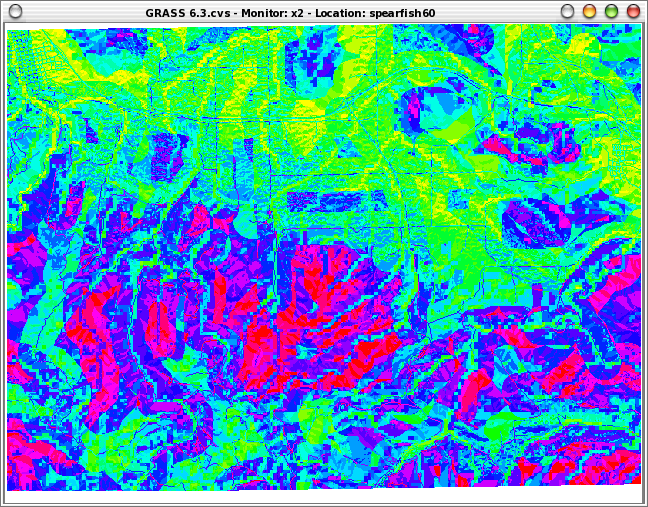
\includegraphics[scale=0.35]{grass021.png}
   %caption of the figure
   \caption{Carte de score}
   %label of the figure, which has to correspond to \ref{}:
   \label{fig:grass021}
\end{figure}

\subsection{METTRE EN BLOC LES ZONES SOUHAITABLES}
ATTENTION: Cette partie demande l'utilisation du prompt/terminal avec des commandes en ligne.

Qu'est-ce que ``mettre en bloc''?
Re-cat\'egoriser les donn\'ees dans une carte raster en groupant les pixels qui form des surfaces continues physiquement en d'uniques cat\'egories.

Maintenant, trouvez les zones discr\`etes/continues (ou clumps) des scores d'aggr\'egation d'habitat. 
Lancez \textit{r.clump (..=>Clump Small Areas) }sur la carte ``\textit{score\_final}'' pour donner \`a chaque bloc son propre num\'ero de cat\'egorie. Vous pourriez appeler la carte r\'esultante ``\textit{score\_clumped}''.

\begin{smallverbatim}
r.clump input=score_final output=score_clumped 
\end{smallverbatim}

Affichez votre nouvelle carte de blocs ``\textit{score\_clumped}''. Elle devrait plus ou moins ressembler \`a cel\`a:Fig.~\ref{fig:grass022}

%\setkeys{Gin}{width=1\textwidth}
\begin{figure}[htbp]
   \centering
   %name of your graphic, without the path AND in PNG (screnshots etc)/PDF (drawings) format:
   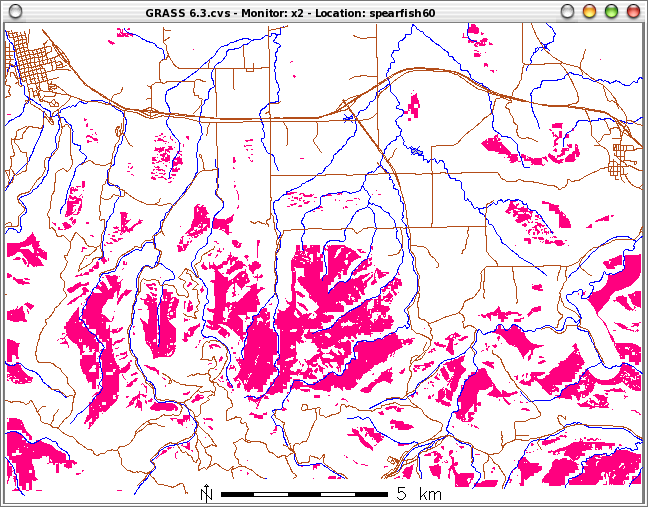
\includegraphics[scale=0.35]{grass022.png}
   %caption of the figure
   \caption{Carte des blocs}
   %label of the figure, which has to correspond to \ref{}:
   \label{fig:grass022}
\end{figure}


Puisque cette esp\`ece est mieux dans de larges blocs, faites une extraction des blocs sup\'erieurs a 50 hectares dans une carte sp\'epar\'ee. Vous pourriez utilisez le terminal pour reclassifier par seuil de surface sup\'erieur \`a 50 hectares:

\begin{smallverbatim}
r.reclass.area input = score_final greater=50 
 output=selected_habitat_area
\end{smallverbatim}

R\'esultat ``selected\_habitat\_area'' \`a ce niveau devrait \^etre similaire \`a ceci:Fig.~\ref{fig:grass023}

%\setkeys{Gin}{width=1\textwidth}
\begin{figure}[htbp]
   \centering
   %name of your graphic, without the path AND in PNG (screnshots etc)/PDF (drawings) format:
   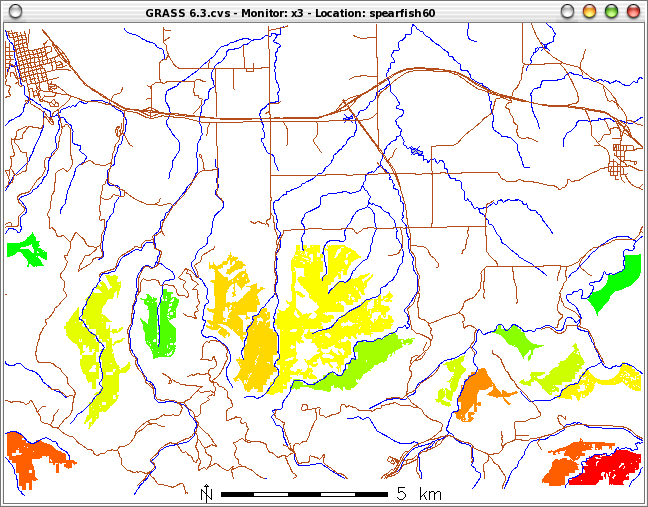
\includegraphics[scale=0.35]{grass023.png}
   %caption of the figure
   \caption{Zones d'habitat s\'electionn\'ees}
   %label of the figure, which has to correspond to \ref{}:
   \label{fig:grass023}
\end{figure}

\subsection{EXPORT DES RESULTATS SOUS FORMAT VECTORIEL}
Puisque nos clients travaillent sous SIG \`a format vectoriel, nous allons convertir les r\'esultats en format vectoriel et les exporter de GRASS \`a ESRI shapefile.

Vectorisez larte de blocs que vous venez de produire (File/Map type conversion/raster to vector) et v\'erifiez que vous avez effectivement cr\'ee une carte vectorielle \`a \'el\'ements de type polygones en affichant votre couche vectorielle avec des couleurs al\'eatoires.Fig.~\ref{fig:grass024}

%\setkeys{Gin}{width=1\textwidth}
\begin{figure}[htbp]
   \centering
   %name of your graphic, without the path AND in PNG (screnshots etc)/PDF (drawings) format:
   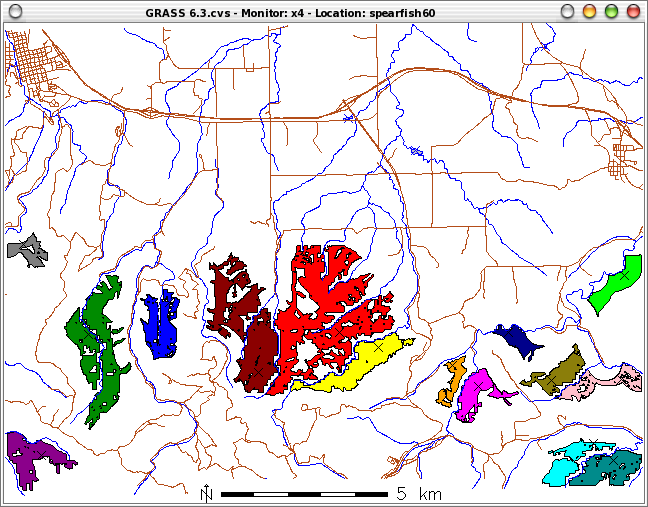
\includegraphics[scale=0.35]{grass024.png}
   %caption of the figure
   \caption{Export de fichier vectoriel}
   %label of the figure, which has to correspond to \ref{}:
   \label{fig:grass024}
\end{figure}

Exportez ce fichier vectoriel d'habitat avec ``\textit{roads}'' et ``\textit{streams}'' aussi en format shapefile. Soyez s\^ur que vous exportez le m\^eme type d'\'el\'ements vectoriels (area pour ``\textit{selected\_habitat\_area}'' et lines pour ``\textit{roads}'' et ``\textit{streams}''). Affichez et questionnez ces fichiers dans le SIG Quantum.

\begin{smallverbatim}
v.out.ogr input=selected_habitat_area type=area
 dsn=QGISDATA layer=1 format=ESRI_Shapefile

v.out.ogr input=roads type=line dsn=QGISDATA
 layer=1 format=ESRI_Shapefile

v.out.ogr input=streams type=line dsn=QGISDATA
 layer=1 format=ESRI_Shapefile
\end{smallverbatim}

Bonus de traitement de donn\'ees.....

Cette esp\`ece est assez intol\'erante des perturbations aux fronti\`eres de zones, donc vous devriez faire un poids plus lourd pour les zones internes que frontali\`eres des blocs d'habitat. Cr\'eez des buffers internes concentriques de 100 m\`etres pour chaque bloc, avec un poids de 1 pour le premier buffer en fronti\`ere (0-100 m\`etres internes), 2 pour le second vers l'interieur (100-200 m\`etres), 3 pour 200-300 m\`etres, etc..., quand aux pixels en dehors des blocs, leurs valeurs sont de z\'ero.

Utilisez \textit{r.mapcalc} pour multiplier la carte d'habitat par les poids des buffers internes.
Maintenant lancez \textit{r.volume }sur cette carte r\'esultante pour obtenir la somme et la moyenne de chaque bloc.
Utilisez  \textit{awk} pour cr\'eer des fichiers de r\`egles de r\'eclassification, puis utilisez \textit{r.reclass} pour cartographier les blocs par somme et moyenne.
Quel bloc a le nouveau total maximum? Lequel a la nouvelle moyenne maximum?
Utilisez \textit{r.grow} pour cr\'eer une carte de fronti\`eres de blocs (soustraire les cartes d'origines aux cartes r\'esultantes).
Utilisez les cartes de fronti\`eres de blocs pour indexer le p\'erimetre de chaque bloc majeur. 
Calculez la compacit\'e (surface divis\'ee par le carr\'e du p\'erimetre) de chaque bloc. 
Cartographiez les blocs par compacit\'e. Cr\'eez un script d'affichage cool pour d\'emontrer vos proc\'edures et expliquez ce que vous avez trouv\'e.
(Pour cel\`a voyez: \href{http://www.udel.edu/johnmack/frec682/script_ideas.html})

Un script de quelques pqrties de cet exercice est dans l'\textbf{Appendice B} \ref{appendixB}.

\newpage

\subsection{Appendice A: Overview of Grass GUI}
\label{appendixA}

Overview of the available commands in the modules:Fig.~\ref{fig:grass025} Fig.~\ref{fig:grass026} Fig.~\ref{fig:grass027}

%\setkeys{Gin}{width=1\textwidth}
\begin{figure}[htbp]
   \centering
   %name of your graphic, without the path AND in PNG (screnshots etc)/PDF (drawings) format:
   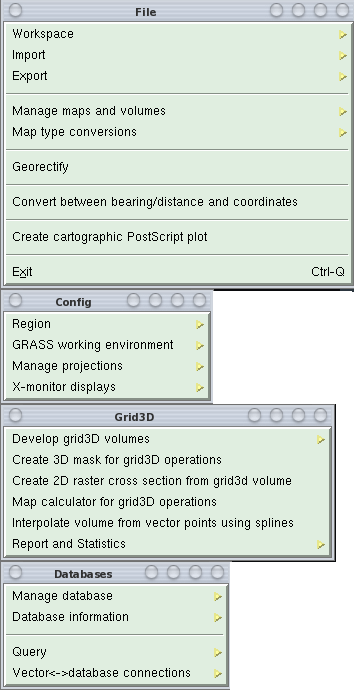
\includegraphics[scale=0.4]{grass025.png}
   %caption of the figure
   \caption{GRASS Menus (1/3)}
   %label of the figure, which has to correspond to \ref{}:
   \label{fig:grass025}
\end{figure}

%\setkeys{Gin}{width=1\textwidth}
\begin{figure}[htbp]
   \centering
   %name of your graphic, without the path AND in PNG (screnshots etc)/PDF (drawings) format:
   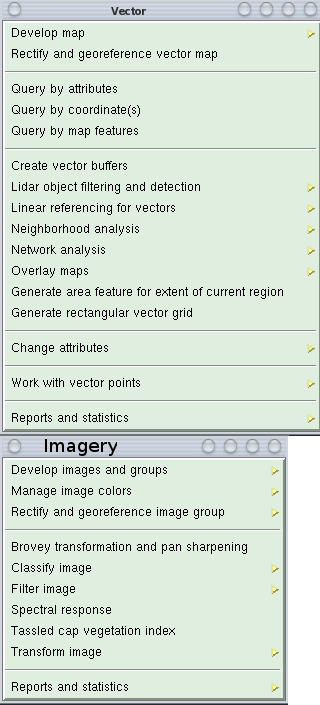
\includegraphics[scale=0.4]{grass026.png}
   %caption of the figure
   \caption{GRASS Menus (2/3)}
   %label of the figure, which has to correspond to \ref{}:
   \label{fig:grass026}
\end{figure}

%\setkeys{Gin}{width=1\textwidth}
\begin{figure}[htbp]
   \centering
   %name of your graphic, without the path AND in PNG (screnshots etc)/PDF (drawings) format:
   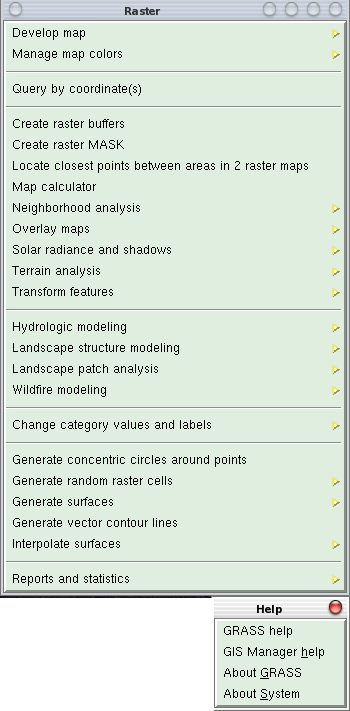
\includegraphics[scale=0.4]{grass027.png}
   %caption of the figure
   \caption{GRASS Menus (3/3)}
   %label of the figure, which has to correspond to \ref{}:
   \label{fig:grass027}
\end{figure}

\newpage

\subsection{Appendix B: GRASS SCRIPT}
\label{appendixB}

Please put this into a file that you may name \textit{script.sh}\textup{and from a }\textit{Terminal}\textup{ type: ``chmod 0755}\textit{script.sh''}\textup{. Then you can run the script }by typing the command: ``./script.sh''.

\begin{smallverbatim}
#!/bin/bash
# main map names variables
dem=elevation.dem
r=roads
s=streams
# buffer streams and roads variables
_bs=_bstreams500
_br=_broads500
# reclassed buffer streams and roads variables
_rbs=_rbstreams500
_rbr=_rbroads500
#--------------------------------------------------
# General Presentation: Start Monitor 0
#--------------------------------------------------
d.mon start=x0
d.erase color=grey
d.rast map=\$dem
sleep 1
d.vect map=\$r color=brown
sleep 1
d.vect map=\$s color=blue
sleep 1
d.barscale bcolor=white tcolor=black at=30.0,95.0
sleep 2
#--------------------------------------------------
# Buffering: Start Monitor 1
#--------------------------------------------------
d.mon start=x1
d.mon select=x1
d.erase color=grey
r.buffer input=\$s output=\$_bs distances=500
 units=meters --overwrite
r.null map=\$_bs null=0
d.rast map=\$_bs
d.vect map=\$s color=blue
d.barscale bcolor=white tcolor=black at=30.0,95.0
r.buffer input=\$r output=\$_br distances=500
 units=meters --overwrite
r.null map=\$_br null=0
d.rast map=\$_br
d.vect map=\$s color=blue
d.barscale bcolor=white tcolor=black at=30.0,95.0
#--------------------------------------------------
# Reclassification: Start Monitor 2
#--------------------------------------------------
d.mon start=x2
d.mon select=x2
d.erase color=grey
echo "...Reclassify..."
r.mapcalc \$_rbs="if(\$_bs==2,1,0)"
r.mapcalc _s_sl="if(\$_rbs==1,if(slope<=5,2,5),0)"
r.mapcalc \$_rbr="float(if(\$_br==2,-5.0,0))"
r.mapcalc _for="if(vegcover==3,4,0)"
r.mapcalc _for1="if(vegcover==5,1,0)"
r.mapcalc _exp1="if(aspect<45.0 || aspect>314.0 &&
 aspect != 0.0,1,0)"
r.mapcalc _exp2="if(aspect<225.0 && aspect>135.
 0,1,0)"
r.mapcalc _exp3="if(aspect<=135.0 && aspect>=45.0,
 3,0)"
r.mapcalc _elev1="if(\$dem<1400 &&\$dem>1200,2,0)"
r.mapcalc _elev2="if(\$dem<1600 &&\$dem>=1400,4,0)"
r.mapcalc _elev3="if(\$dem>=1600,2,0)"
#--------------------------------------------------
r.buffer input=\$r output=_br100 distances=100
 units=meters --overwrite
r.null map=\_br100 null=0
r.mapcalc _add="float(_s_sl+\$_rbr+_for+_for1+
 _exp1+_exp2+_exp3+_elev1+_elev2+_elev3)"
r.mapcalc _clas="if(_add{>9,1,null())"
r.mapcalc _class="if(_clas==1&&_br100==0,1,null())"
echo "Reclassification...done."
d.rast map="\$_rbs"
sleep 1
d.rast map="_s_sl"
d.rast map="\$_rbr"
d.rast map="_for"
d.rast map="_for1"
d.rast map="_exp1"
d.rast map="_exp2"
d.rast map="_exp3"
d.rast map="_elev1"
d.rast map="_elev2"
d.rast map="_elev3"
d.rast map="_br100"
sleep 1
#r.colors color=grey map="_add"
d.rast map="_add"
sleep 1
d.rast map="_class"
sleep 1
#d.erase
d.vect map="\$s" color=blue
d.vect map="\$r" color=brown
d.barscale bcolor=white tcolor=black at=30.0,95.0
sleep 5
g.remove
rast="\$_rbs,_s_sl,\$_rbr,_for,_for1"}
g.remove
rast="_exp1,_exp2,_exp3,_elev1"}
g.remove
rast="_elev2,_elev3,_br100,_add"}
g.remove rast="\$_bs,\$_br,_clas"}
sleep 1
echo ""
echo "finished"
sleep 1
#--------------------------------------------------
# Clumping: Start Monitor 3
#--------------------------------------------------
d.mon start=x3
d.mon select=x3
d.erase color=grey
g.remove rast=_clump.clump._rclumpnew
r.clump input=_class output=_clump --overwrite
r.colors color=gyr map="_clump"
d.rast map="_clump"
sleep 1
r.reclass.area input=_clump greater=50
 output=_rclumpnew --overwrite
r.colors color=gyr map="_rclumpnew"
d.erase color=white
d.rast map="_rclumpnew"
sleep 1
d.vect map="streams" color=blue
d.vect map="roads" color=brown
d.barscale bcolor=white tcolor=black at=30.0,95.0
sleep 1
g.remove rast="_clump,_class"
#--------------------------------------------------
# R2V and Export: Start Monitor 4
#--------------------------------------------------
d.mon start=x4
d.mon select=x4
d.erase color=white
r.to.vect -s input=_rclumpnew output=rclump
 feature=area --overwrite
d.vect -c map=rclump type=area color=black
d.vect map="streams" color=blue
d.vect map="roads" color=brown
d.barscale bcolor=white tcolor=black at=30.0,95.0
sleep 1
v.out.ogr input=rclump type=area dsn=QGISDATA
 layer=1 format=ESRI_Shapefile --overwrite
g.remove rast="_rclumpnew"
g.remove vect="rclump"
d.mon stop=x4
d.mon stop=x3
d.mon stop=x2
d.mon stop=x1
d.mon stop=x0
\end{smallverbatim}

\address{GRASS Development Team\\
  \url{http://grass.itc.it}\\
  \email{weblist@grass.itc.it}}

%%% Local Variables: 
%%% mode: latex
%%% TeX-master: main_document.tex
%%% End: 

